\documentclass[12pt,a4paper]{jarticle}
\usepackage[dvipdfmx]{graphicx}
\usepackage[margin=10truemm]{geometry}
\graphicspath{{../png/}}
\begin{document}
\section{塩分変化のコンター,以下すべて河川流量1倍}
\begin{figure}[hbtp]
    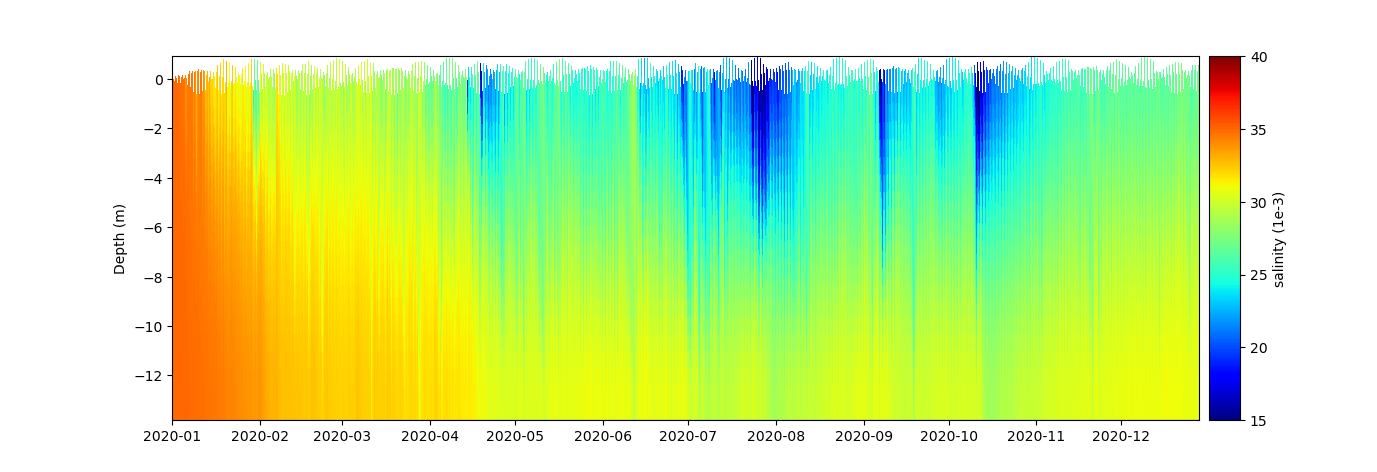
\includegraphics[keepaspectratio,width=180mm]{contour/Tokyo6_chiba1buoy.png}
    \caption{河川流量1倍 chiba1buoy}
\end{figure}

%\section{河川流量1倍時のsigma layerごとでの水温変化,中小河川入力済み,chiba1buoy}
\begin{figure}[hbtp]
    \begin{tabular}{cc}
      \begin{minipage}[t]{0.3\hsize}
        \centering
        \includegraphics[keepaspectratio, width=50mm]{Tokyo6/salinity_chiba1buoy_2_Tokyo6.png}
        \caption{siglay=2,chiba1buoy}
      \end{minipage} &
      \begin{minipage}[t]{0.3\hsize}
        \centering
        \includegraphics[keepaspectratio, width=50mm]{Tokyo6/salinity_chiba1buoy_10_Tokyo6.png}
        \caption{siglalay=10,chiba1buoy}
      \end{minipage} 
      \begin{minipage}[t]{0.3\hsize}
        \centering
        \includegraphics[keepaspectratio, width=50mm]{Tokyo6/salinity_chiba1buoy_18_Tokyo6.png}
        \caption{siglay=18,chiba1buoy}
      \end{minipage}
    \end{tabular}
  \end{figure}

%\section{河川流量1倍時のsigma layerごとでの水温変化/中小河川入力済み/chibaharo}
\begin{figure}[hbtp]
    \begin{tabular}{cc}
      \begin{minipage}[t]{0.3\hsize}
        \centering
        \includegraphics[keepaspectratio, width=50mm]{Tokyo6/salinity_chibaharo_2_Tokyo6.png}
        \caption{siglay=2,chibaharo}
      \end{minipage} &
      \begin{minipage}[t]{0.3\hsize}
        \centering
        \includegraphics[keepaspectratio, width=50mm]{Tokyo6/salinity_chibaharo_10_Tokyo6.png}
        \caption{siglalay=10,chibaharo}
      \end{minipage} 
      \begin{minipage}[t]{0.3\hsize}
        \centering
        \includegraphics[keepaspectratio, width=50mm]{Tokyo6/salinity_chibaharo_18_Tokyo6.png}
        \caption{siglay=18,chibaharo}
      \end{minipage}
    \end{tabular}
  \end{figure}

  %\section{河川流量1倍時のsigma layerごとでの水温変化/中小河川入力済み/urayasu}
  \begin{figure}[hbtp]
      \begin{tabular}{cc}
        \begin{minipage}[t]{0.3\hsize}
          \centering
          \includegraphics[keepaspectratio, width=50mm]{Tokyo6/salinity_urayasu_2_Tokyo6.png}
          \caption{siglay=2,urayasu}
        \end{minipage} &
        \begin{minipage}[t]{0.3\hsize}
          \centering
          \includegraphics[keepaspectratio, width=50mm]{Tokyo6/salinity_urayasu_10_Tokyo6.png}
          \caption{siglalay=10,urayasu}
        \end{minipage} 
        \begin{minipage}[t]{0.3\hsize}
          \centering
          \includegraphics[keepaspectratio, width=50mm]{Tokyo6/salinity_urayasu_18_Tokyo6.png}
          \caption{siglay=18,urayasu}
        \end{minipage}
      \end{tabular}
    \end{figure}

    %\section{河川流量1倍時のsigma layerごとでの水温変化/中小河川入力済み/kawasaki}
    \begin{figure}[hbtp]
        \begin{tabular}{cc}
          \begin{minipage}[t]{0.3\hsize}
            \centering
            \includegraphics[keepaspectratio, width=50mm]{Tokyo6/salinity_kawasaki_2_Tokyo6.png}
            \caption{siglay=2}
          \end{minipage} &
          \begin{minipage}[t]{0.3\hsize}
            \centering
            \includegraphics[keepaspectratio, width=50mm]{Tokyo6/salinity_kawasaki_10_Tokyo6.png}
            \caption{siglalay=10}
          \end{minipage} 
          \begin{minipage}[t]{0.3\hsize}
            \centering
            \includegraphics[keepaspectratio, width=50mm]{Tokyo6/salinity_kawasaki_18_Tokyo6.png}
            \caption{siglay=18}
          \end{minipage}
        \end{tabular}
      \end{figure}

    \end{document}
